\documentclass[10pt]{article}
\usepackage[top=2.5cm, bottom=3cm, left=2.3cm, right=2.3cm]{geometry}
\usepackage{graphicx}
\usepackage{subfigure}
\usepackage{psfrag}
\usepackage{amsmath}
\usepackage{natbib}
\usepackage{color}
\usepackage[normalem]{ulem}
\usepackage{csquotes}
\usepackage{cleveref}
\usepackage{epstopdf, epsfig}
\usepackage{wrapfig}
\usepackage{amsbsy}
\usepackage{lineno,hyperref}
\usepackage{verbatim}

\def\lp{\left(}
\def\rp{\right)}
\def\tp{\overline{{\theta^\prime}^2}}
\def\tm{\overline{\theta}}
\def\tr{{\theta^\prime}}

\begin{document}
\section*{Radiative modification to a general $\tp - \epsilon_{\theta}$ model}
\vspace{1cm}
Quantities requiring modeling:

\begin{equation*}
\kappa^\prime \ , \ \ \ E_m^\prime \ , \ \ \ G^\prime \ .
\end{equation*}
They all depend on temperature (Radiative heat transfer is an analytical equation), in particular we know that:
\begin{equation*}
\kappa = c_0 + \frac{c_1}{T} + \frac{c_2}{T^2} + \frac{c_3}{T^3} + \frac{c_4}{T^4} + \frac{c_5}{T^5} \ ,
\end{equation*}
and
\begin{equation*}
E_m = 4 {\lp \frac{\theta}{T_0} + 1\rp }^4 \ ,
\end{equation*}
where:
\begin{equation*}
T = \theta \Delta T + T_c \ ,  \ \ \ \ \overline{T} = \tm \Delta T+ T_c \ , \ \ \ \ T^\prime = \tr \Delta T \ , \ \ \ \ T_0 = \frac{T_c}{\Delta T} \ .
\end{equation*}
\subsection*{Approximation of $E_m^\prime$}
It is possible to find the fluctuation of these two quantities by linearizing their analytical expressions, starting from $E_m$
\begin{equation*}
E_m^\prime  = E_m - \overline{E_m} = 4 {\lp \frac{\theta}{T_0} + 1\rp }^4 - 4\overline{ {\lp \frac{\theta}{T_0} + 1\rp }^4}
\end{equation*}
\begin{equation*}
E_m^\prime  = \frac{4 \theta^4}{T_0^4} + \frac{16 \theta^3}{T_0^3} + \frac{24 \theta^2}{T_0^2} + \frac{16\theta}{T_0}  
            - \frac{4 \overline{\theta^4}}{T_0^4} - \frac{16 \overline{\theta^3}}{T_0^3} - \frac{24 \overline{\theta^2}}{T_0^2} - \frac{16\tm}{T_0}  
\end{equation*}
after subtituting $\theta$ with $\tr+\tm$
\begin{equation*}
\begin{split}
E_m^\prime & = \frac{4 (\tm^4 + 4\tm^3 \tr + 6\tm^2 \tr^2+4\tm\tr^3+\tr^4)}{T_0^4} + \frac{16 (\tm^3 + 3\tm^2\tr+3\tm\tr^2+\tr^3)}{T_0^3} + \frac{24 (\tm^2+2\tm\tr+\tr^2)}{T_0^2} + \frac{16(\tm+\tr)}{T_0} + \\
           & - \frac{4 (\tm^4 + 6\tm^2 \tp +4\tm\overline{\tr^3} + \overline{\tr^4})}{T_0^4} - \frac{16(\tm^3 +3\tm\tp+\overline{\tr^3})}{T_0^3} - \frac{24 \tm^2 + \tp}{T_0^2} - \frac{16\tm}{T_0}  \ ,
\end{split}
\end{equation*}
\begin{equation*}
\begin{split}
E_m^\prime & = \frac{4 (4\tm^3 \tr + 6\tm^2 (\tr^2-\tp)+4\tm(\tr^3-\overline{\tr^3})+\tr^4-\overline{\tr^4})}{T_0^4} + \frac{16 (3\tm^2\tr+3\tm(\tr^2-\tp)+\tr^3-\overline{\tr^3})}{T_0^3} + \\
           & + \frac{24 (2\tm\tr+\tr^2-\tp)}{T_0^2} + \frac{16(\tr)}{T_0}  \ .
\end{split}
\end{equation*}
In the end, simplifying and underlying the dependency on temperature fluctuations $\tr$:
\begin{equation*}
\begin{split}
E_m^\prime & = \lp \frac{16 \tm^3}{T_0^4} + \frac{48 \tm^2}{T_0^3} + \frac{48 \tm}{T_0^2} + \frac{16}{T_0}  \rp \tr + \\
           & = \lp \frac{24 \tm^2}{T_0^4} + \frac{48 \tm}{T_0^3}   + \frac{24}{T_0^2}   \rp (\tr^2 - \tp) + \\
           & = \lp \frac{16 \tm}{T_0^4}   + \frac{16} {T_0^3}   \rp (\tr^3 - \overline{\tr^3}) + \\
           & = \lp \frac{4}{T_0^4}  \rp (\tr^4 - \overline{\tr^4})  \ .
\end{split}
\end{equation*}
Due to the linearization we can neglect all terms depending on higher order terms, therefore in the end a good approximation for $E_m^\prime$ is
\begin{equation*}
E_m^\prime \approx f_{E_m} \theta^\prime \ ,
\end{equation*}
where $f_{E_m}$ is the first model equation, equal to:
\begin{equation*}
f_{E_m} =  \frac{16 \tm^3}{T_0^4} + \frac{48 \tm^2}{T_0^3} + \frac{48 \tm}{T_0^2} + \frac{16}{T_0} \ .
\end{equation*}

\subsection*{Approximation of $\kappa^\prime$ (only for variable $\kappa$)}
To calculate $\kappa^\prime$ is necessary to calculate $\overline{\kappa}$ first as $\kappa^\prime = \kappa - \overline{\kappa}$.
\begin{equation*}
\overline{\kappa} = c_0 + \overline{\frac{c_1}{T}} + \overline{\frac{c_2}{T^2}} + \overline{\frac{c_3}{T^3}} + \overline{\frac{c_4}{T^4}} + \overline{\frac{c_5}{T^5}} \ ,
\end{equation*}
taking into account the second term on the LHS, (remembering that $c_1$ is a constant):
\begin{equation*}
\overline{\frac{1}{T}} = \overline{\frac{1}{\overline{T}(1+\frac{T^\prime}{\overline{T}})}} \ ,
\end{equation*}
since $T^\prime/\overline{T} \ll 1$ it is possible taking a taylor expansion ${(1+x)^{-1} = 1-x+x^2-x^3 ...}$ and linearize, therefore:
\begin{equation*}
\overline{\frac{1}{T}} \approx \overline{\frac{1}{\overline{T}}(1 - \frac{T^\prime}{\overline{T}})} = \frac{1}{\overline{T}} \ .
\end{equation*}
Proceding with the same logic it is possible to show that, if $T^\prime/\overline{T} \ll 1$, then:
\begin{equation*}
\overline{\frac{1}{T^2}} \approx \frac{1}{\overline{T^2}} \ , \ \ \ \overline{\frac{1}{T^3}} \approx \frac{1}{\overline{T^3}} \ , \ \ \ \overline{\frac{1}{T^4}} \approx \frac{1}{\overline{T^4}} \ , \ \ \ \overline{\frac{1}{T^5}} \approx \frac{1}{\overline{T^5}} \ .  
\end{equation*}
Therefore
\begin{equation*}
\overline{\kappa} \approx c_0 + \frac{c_1}{\overline{T}} + \frac{c_2}{\overline{T^2}} + \frac{c_3}{\overline{T^3}} + \frac{c_4}{\overline{T^4}} + \frac{c_5}{\overline{T^5}} \ .
\end{equation*}
To calculate $\kappa^\prime$ we start from the second term on the LHS ($c_0 - c_0 = 0$)
\begin{equation*}
c_1 \lp \frac{1}{T} - \frac{1}{\overline{T}} \rp = c_1 \lp \frac{\overline{T} - T}{T\overline{T}} \rp \ .
\end{equation*}
Substituting the expressions $T^\prime  = T - \overline{T} = \theta^\prime \Delta T$ and linearizing the denominator ($T\overline{T} \approx \overline{T}^2$)
\begin{equation*}
c_1 \lp \frac{1}{T} - \frac{1}{\overline{T}} \rp \approx - c_1 \frac{\Delta T}{\overline{T}^2} \tr \ .
\end{equation*}
For the third term, subtracting and expanding into $\overline{T}+T^\prime$
\begin{equation*}
c_2 \lp \frac{1}{T^2} - \frac{1}{\overline{T^2}} \rp = c_2 \lp \frac{\overline{{T^\prime}^2} - 2\overline{T}{T^\prime} - {T^\prime}^2}{(\overline{T}^2 + 2\overline{T}T^\prime + {T^\prime}^2)(\overline{T}^2 + \overline{{T^\prime}^2)}} \rp \ .
\end{equation*}
Again linearizing the denominator ($\approx \overline{T}^4$) and the numerator ($\approx 2\overline{T}T^\prime$) we reach
\begin{equation*}
c_2 \lp \frac{1}{T^2} - \frac{1}{\overline{T^2}} \rp \approx - c_2  \frac{2\Delta T}{\overline{T}^3} \tr \ .
\end{equation*}
In the same fashion it is possible to demonstrate that 
\begin{equation*}
\begin{split}
c_3 \lp \frac{1}{T^3} - \frac{1}{\overline{T^3}} \rp & \approx - c_3  \frac{3\Delta T}{\overline{T}^4} \tr \ ,\\
c_4 \lp \frac{1}{T^4} - \frac{1}{\overline{T^4}} \rp & \approx - c_4  \frac{4\Delta T}{\overline{T}^5} \tr \ ,\\
c_5 \lp \frac{1}{T^5} - \frac{1}{\overline{T^5}} \rp & \approx - c_5  \frac{5\Delta T}{\overline{T}^6} \tr \ .
\end{split}
\end{equation*}
And therefore we found an expression for $\kappa^\prime$ as
\begin{equation*}
\kappa^\prime \approx f_{\kappa} \theta^\prime \ ,
\end{equation*}
where
\begin{equation*}
f_{\kappa} =  - \lp c_1  \frac{\Delta T}{\overline{T}^2} + c_2  \frac{2\Delta T}{\overline{T}^3} + c_3  \frac{3\Delta T}{\overline{T}^4} +  c_4  \frac{4\Delta T}{\overline{T}^4} +  c_5  \frac{5\Delta T}{\overline{T}^6} \rp
\end{equation*}
\subsection*{Approximation of $G^\prime$}
This is the most complex part of the modeling and 

\begin{figure}[h]
\centering
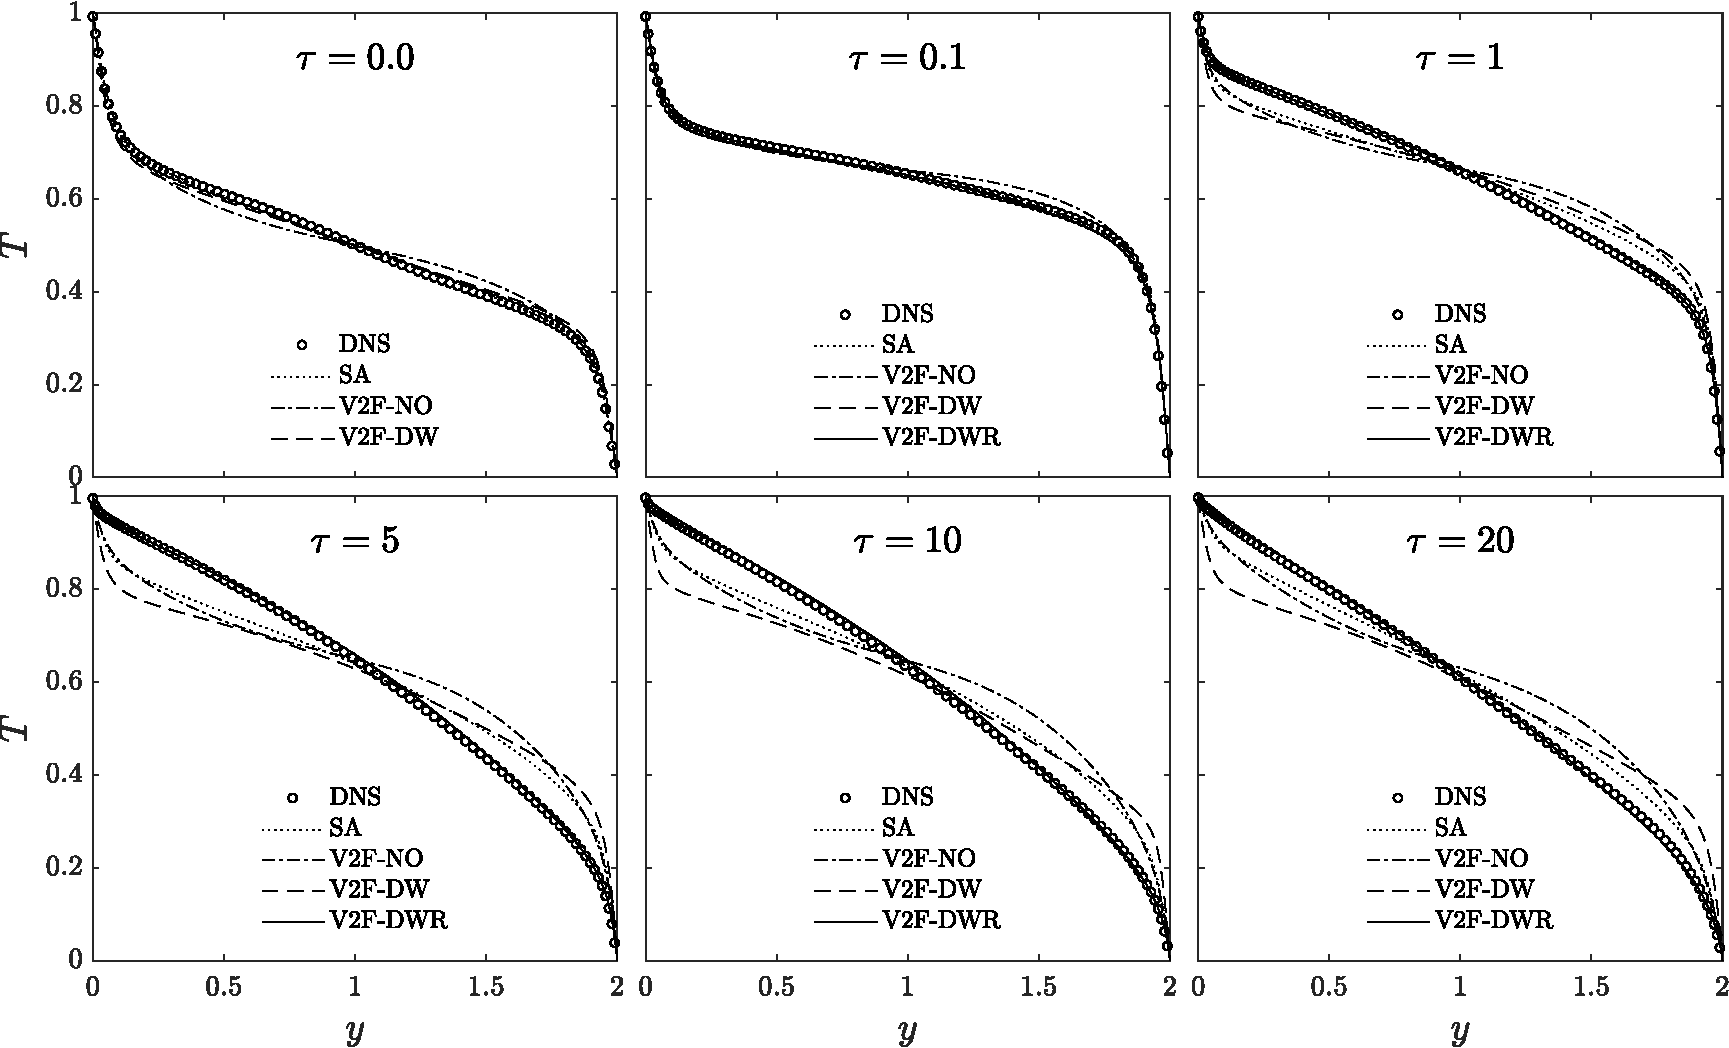
\includegraphics[width=1.1\textwidth]{../solution/Figures/Tempgrey.pdf}
\caption{\noindent RANS simulation with different turbulent heat flux models for different $\tau$ cases}
\label{constk}
\end{figure}

\begin{figure}[h]
\centering
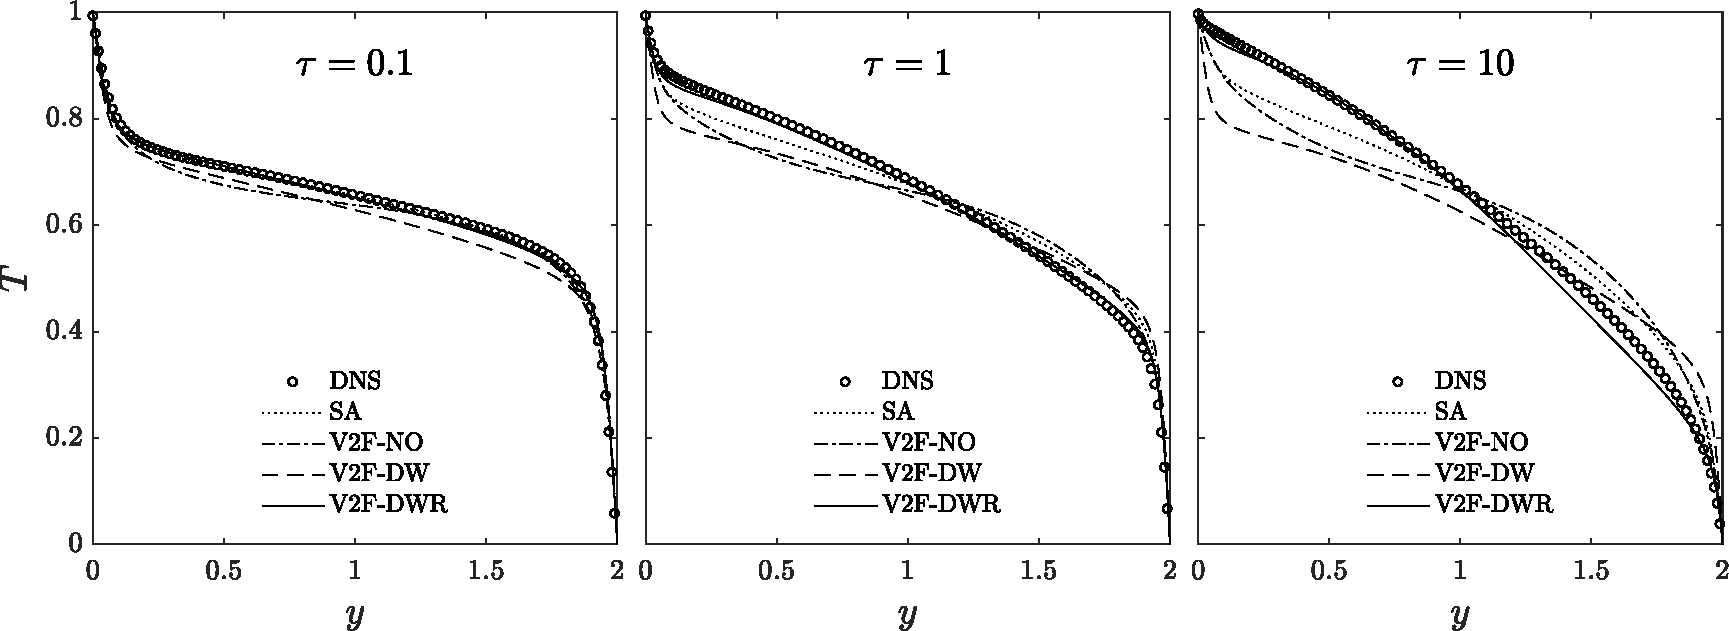
\includegraphics[width=1.1\textwidth]{../solution/Figures_r/Tempvar.pdf}
\caption{\noindent RANS simulation with different turbulent heat flux models for different $\tau$ cases}
\label{vark}
\end{figure}


\end{document}
